\documentclass[11pt]{article}
\usepackage[T1]{fontenc}
\usepackage{lmodern}
\usepackage{amsmath,amssymb,amsthm,mathtools}
\usepackage[margin=1in]{geometry}
\usepackage{microtype}
\usepackage{enumitem,needspace,float}
\usepackage{tikz}
\usetikzlibrary{arrows.meta,positioning,calc,decorations.pathreplacing}
\usepackage{xcolor}
\definecolor{linkblue}{RGB}{25,65,100}
\usepackage[colorlinks=true,linkcolor=linkblue,citecolor=linkblue,urlcolor=linkblue]{hyperref}
\hypersetup{pdftitle={The sharp terminal leave in random triangle removal},pdfauthor={OpenAI}}
\pdfinfoomitdate=1
\pdftrailerid{}
\pdfsuppressptexinfo=15
\newtheorem{theorem}{Theorem}[section]
\newtheorem{proposition}[theorem]{Proposition}
\newtheorem{lemma}[theorem]{Lemma}
\newtheorem{corollary}[theorem]{Corollary}
\theoremstyle{definition}
\newtheorem{definition}[theorem]{Definition}
\theoremstyle{remark}
\newtheorem{remark}[theorem]{Remark}
\newcommand{\E}{\mathbb E}
\newcommand{\Prb}{\mathbb P}
\newcommand{\cE}{\mathcal E}
\newcommand{\cT}{\mathcal T}
\numberwithin{equation}{section}
\setlist{topsep=5pt,itemsep=3pt,parsep=0pt}
\setcounter{tocdepth}{2}
\allowdisplaybreaks[1]
\emergencystretch=1em


\title{The sharp terminal leave in random triangle removal}
\author{OpenAI}
\date{September 25, 2026}
\begin{document}
\maketitle
\begin{abstract}
Starting from the complete graph on $n$ vertices, repeatedly remove the three
edges of a uniformly chosen remaining triangle. We prove that the number of
edges left at termination, divided by $n^{3/2}$, converges in $L^2$ to
$1/(2\sqrt2)$. This proves the triangle case of the sharp-constant conjecture
of Joos and K\"uhn. In particular, the same limit holds in probability and
for the normalized expectation.
\end{abstract}
\tableofcontents
\clearpage
\section{Introduction}
\label{sec:introduction}

Begin with the complete graph $K_n$. At each step, choose uniformly from
the triangles whose three edges are still present, and delete those edges.
Stop when no triangle remains. The removed triangles form an edge-disjoint
packing; the edges left over form its \emph{leave}. Let $F_n$ be the number
of edges in this terminal graph. The problem is to determine the typical
size of this leave, including its leading constant.

The accepted triangles form a partial Steiner triple system, and $F_n$
measures its uncovered pairs. Bollob\'as and Erd\H{o}s conjectured in 1990
that the expected leave has order $n^{3/2}$, as reported in
\cite[Introduction]{BohmanFriezeLubetzky2015}.
Spencer's branching-process analysis and the independent nibble argument
of R\"odl and Thoma showed that the leave is $o(n^2)$ with high probability
\cite{Spencer1995,RodlThoma1996}. Grable proved bounds
$O(n^{11/6+\xi})$ for each fixed $\xi>0$ and outlined the higher-order
calculations leading to $O(n^{7/4+\xi})$
\cite[Theorems~5 and~7]{Grable1997}.
Bohman, Frieze and Lubetzky gave a short proof of the bound
$O(n^{7/4}\log^{5/4}n)$ \cite[Theorem~1]{BohmanFriezeLubetzky2010}
and subsequently proved $F_n=n^{3/2+o(1)}$ with high probability
\cite[Theorem~1]{BohmanFriezeLubetzky2015}. Their analysis uses
self-correcting dynamic concentration and carefully chosen triangular
extensions to determine the exponent.

Joos and K\"uhn developed removal estimates for general strictly balanced
hypergraphs, including pseudorandom starting hypergraphs
\cite[Theorems~1.2--1.3]{joosKuehn2025}. Their Conjecture~16.2 predicts
an asymptotic constant for the terminal leave; its triangle specialization
is $1/(2\sqrt2)$ in probability. The following theorem proves this
triangle case with $L^2$ convergence. Numbered references to Joos and
K\"uhn refer throughout to version~2.

\begin{theorem}\label{thm:main}
For the uniform triangle-removal process starting from $K_n$,
\[
 \E\left[\left(\frac{F_n}{n^{3/2}}-
                   \frac1{2\sqrt2}\right)^2\right]\longrightarrow0.
\]
In particular,
\[
 \frac{F_n}{n^{3/2}}\xrightarrow{\Prb}\frac1{2\sqrt2},
 \qquad
 \frac{\E F_n}{n^{3/2}}\longrightarrow\frac1{2\sqrt2}.
\]
\end{theorem}

The only external proof input is the early-prefix control from
Joos and K\"uhn, specialized in Section~\ref{sec:prefix}. All subsequent
continuation estimates are proved here. The theorem concerns removal
from $K_n$; it does not assert a sharp constant for arbitrary starting
graphs or for general hypergraph removal, or a fluctuation law.

\subsection{The continuation argument}

The proof separates the part of the process governed by uniform subgraph
counts from the final evolution of individual edges. Stop at a deterministic
time when the edge density is approximately $p=n^{-1/2+\epsilon}$, for a
small fixed $\epsilon>0$. The graph then has
\[
 m=\frac{n^2p}{2}\quad\text{edges},\qquad D=np^2
\]
triangles through each edge to relative error $o(1)$.
Section~\ref{sec:prefix} states the exact properties needed and verifies
their application from the public removal estimates.

The continuation analysis uses backward priority exploration, whose
hypergraph form appears in Spencer's work
\cite[Sections~2--4]{Spencer1995}. Grable formulated triangle packing
as a uniform priority scan and used adaptive exposure decision trees in
his concentration analysis
\cite[Sections~1 and~4]{Grable1997}. The quantitative issue here is to
follow a growing rescaled time interval and to approximate joint survival
on the scale of its vanishing probability. A fixed-time local
approximation alone does not give the precision required for a second
moment.

Give the triangles of this graph fresh independent uniform priorities and
scan them in increasing order, accepting a triangle when all its edges
remain. This represents the continuation of uniform removal. An edge
survives precisely when a recursive test returns true. A child test asks
whether the other \emph{two} edges of a candidate triangle survive before
its priority. We test the two edges with one jointly ordered list of
candidates, which is essential to the later visitation estimate.
Section~\ref{sec:queries} proves this rule and constructs
an auxiliary tree in which each occurrence of a candidate receives an
independent priority.

In this independent model, the survival probabilities satisfy exact
product equations. The scalar comparison is
\[
 q(t)=(1+2Dt)^{-1/2},\qquad 0\le t\le1.
\]
This is Spencer's scalar branching law after the time change $c=Dt$
\cite[Section~3, equation~(9)]{Spencer1995}. Bal and Bennett obtained
related matching estimates for fixed-degree random regular hypergraphs
and regular hypergraphs of growing girth
\cite[Corollaries~3--4]{BalBennett2023}; here $D$ grows with $n$,
and the terminal rescaled time is $D$.
To prove a uniform approximation by $q$, one needs stability of a matrix
acting on the graph's edges. We obtain it from cycle counts in vertex
links. Each normalized link matrix is close in Euclidean norm to its
averaging projection; the sum of these projections has a directly
controlled semigroup in the maximum norm. A finite perturbation expansion
then gives the stability needed by the product equations
(Section~\ref{sec:stability}).

The final issue is the difference between independent occurrences and
repeated triangle types in the finite graph. We compare the complete
candidate lists exposed by one or two root queries. A repetition forces
an extra graph edge in the union of at most two ancestral query paths
(Section~\ref{sec:coupling}). Small rooted-template bounds control the
number of such witnesses. Joint time ordering controls the probability
that their calls are visited. Their combination gives an absolute error
$o(1/D)$ (Section~\ref{sec:witnesses}). This precision matters because the
two-root survival probability is itself of order $1/D$.

The one- and two-root probabilities determine the first and second
moments of $F_n$. Their normalization is
\[
 mq(1)=\frac{n^2p}{2\sqrt{1+2np^2}}
       \sim\frac{n^{3/2}}{2\sqrt2}.
\]
Uniformity over the good prefix graphs, together with a sufficiently
small prefix failure probability, gives the unconditional conclusion
in Section~\ref{sec:moments}.

The continuation estimates developed here are the maximum-norm stability
of the unfolding and the smaller than $D^{-1}$ error for adaptive paired
queries. Both the numerical constant and the moment conclusion use
these estimates.

\subsection{Conventions}

All graphs are finite and simple. An embedding is injective and preserves
edges; it need not preserve nonedges. Thus an embedding of a fixed labeled
cycle counts its ordered vertex labels, without division by automorphisms.
The notation $(1\pm a)b$ means a number in $[(1-a)b,(1+a)b]$.
All unspecified constants below are independent of $n$ and of the realized
good prefix graph. They may depend on the fixed parameters introduced
next. A statement holds with superpolynomially high probability if its
failure probability is $n^{-\omega(1)}$, meaning smaller than $n^{-C}$
for every fixed $C>0$ when $n$ is sufficiently large.

\section{A uniform early prefix}
\label{sec:prefix}

This section supplies all the graph properties used in the continuation.
In addition to degrees and link cycles, we need two upper bounds for
small rooted graphs. The second is useful when all the remaining choices
together have expected count below one.

Fix
\begin{equation}\label{eq:constants}
 \epsilon=\frac1{2000},\qquad r_0=8000,\qquad
 L=100,\qquad B=50,\qquad
 H_0=\max\{r_0+1,3L+2\}=8001.
\end{equation}
Here $r_0$ and $H_0$ bound the link-cycle lengths and template orders
controlled by the prefix; $L$ and $B$ are fixed for the collision-witness
count in Section~\ref{sec:witnesses}.
Write $G_i$ for the graph after $i$ removals, provided that step is reached,
and put
\begin{align}
 p_i&=1-\frac1n-\frac{6i}{n^2},\notag\\
 i_0&=\left\lfloor\frac{n^2}{6}
             \left(1-\frac1n-n^{-1/2+\epsilon}\right)\right\rfloor,
 \qquad p=p_{i_0},\qquad D=np^2,\qquad m=\frac{n^2p}{2}.
 \label{eq:prefix-time}
\end{align}
These quantities are deterministic. In particular,
\begin{equation}\label{eq:scales}
 p=n^{-1/2+\epsilon}+O(n^{-2}),\qquad
 D\sim n^{2\epsilon},\qquad e(G_{i_0})=m
\end{equation}
whenever $i_0$ is reached.

\begin{definition}[Rooted templates]\label{def:template}
A template $(H,I)$ consists of a graph $H$ and an independent set
$I\subseteq V(H)$ of distinguished vertices. For an injection
$\psi:I\to[n]$, let $X_{H,I,\psi}(G)$ count its edge-preserving injective
extensions to $V(H)$ in $G$. Its scaling at density $p$ is
\[
 S(H,I)=n^{v(H)-|I|}p^{e(H)}.
\]
A subtemplate with the same distinguished set is any subgraph
$H'\subseteq H$ whose vertex set contains $I$, distinguished by $I$.
When $v(H)>|I|$, the rooted density is $e(H)/(v(H)-|I|)$; it is zero
when there are no free vertices. The template is \emph{balanced} if
every same-root subtemplate has rooted density at most that of $(H,I)$.
\end{definition}

The independence of $I$ is a property of the template. Its prescribed
images may have additional edges in $G$.

\begin{proposition}[Good prefix]\label{prop:prefix}
There are constants $c>0$ and $C_0<\infty$ and an event $\mathcal G_n$
measurable from the process through step $i_0$ such that
\[
 \Prb(\mathcal G_n^c)\le
       \exp\bigl(- (\log n)^{4/3}\bigr)=n^{-\omega(1)}
\]
for all sufficiently large $n$. On this event, $i_0$ is reached and
$G=G_{i_0}$ has $m$ edges and the following simultaneous properties.
\begin{enumerate}[label=\textup{(\roman*)}]
\item\label{it:degrees}
Every vertex has degree $(1\pm n^{-c})np$, and every two distinct
vertices have $(1\pm n^{-c})D$ common neighbors.
\item\label{it:cycles}
For every vertex $u$ and $3\le j\le r_0$, the number of embeddings of a
fixed labeled cycle $C_j$ into the link $G[N_G(u)]$ is
$(1\pm n^{-c})D^j$.
\item\label{it:templates}
For every template $(H,I)$ with $v(H)\le H_0$ and every injection
$\psi:I\to[n]$, the following two bounds hold.
If $S(H',I)\ge1$ for every same-root subtemplate $H'$, then
\begin{equation}\label{eq:template-large}
 X_{H,I,\psi}(G)\le(1+\log n)^{C_0}S(H,I).
\end{equation}
If $n^{v(H)-|J|}p^{e(H)-e(H[J])}\le1$ for every
$I\subseteq J\subseteq V(H)$, then
\begin{equation}\label{eq:template-small}
 X_{H,I,\psi}(G)\le(1+\log n)^{C_0}.
\end{equation}
\end{enumerate}
All constants and bounds are uniform over the graph and the prescribed
root images.
\end{proposition}

\begin{proof}
We give the specialization of Joos--K\"uhn's stopping estimates, including
the parameters and rooted conventions. Their Sections~5--7 (pp.~9--11)
set up the trajectories and stopping times; Lemma~10.1 (p.~50) controls
those times, and Lemma~7.15 (pp.~16--17) supplies the two general extension bounds
\cite{joosKuehn2025}.

\paragraph{Public parameters and initial hypotheses.}
Denote their small parameter by $\eta$, keeping it distinct from
$\epsilon$ in \eqref{eq:constants}. Choose $\eta$ small enough for their
hierarchy and so that
\[
 \eta<\epsilon/2,\qquad \eta^{-4}\ge H_0.
\]
Choose their $\delta>0$ sufficiently small in terms of $\eta$, with
$\delta<1/2$. These choices remain fixed as $n$ grows.
The removed graph is a triangle, with uniformity parameter $k=2$ and
2-density $(3-1)/(3-2)=2$; it is strictly 2-balanced.
The initial density in their normalization is
$\theta=2e(K_n)/n^2=1-1/n$. Their density trajectory is therefore exactly
$p_i$ in \eqref{eq:prefix-time}. Their horizon has density
$n^{-1/2+\eta}$, strictly below $p_{i_0}$ for large $n$.

Their Section~5 requires an $(\eta^4,\delta,2)$-pseudorandom initial
graph. For completeness, $K_n$ satisfies all its defining conditions
(P1)--(P4) on p.~3. The public convention permits edges among
distinguished vertices and ignores them in both counts and scalings.
For a template with $r$ distinguished vertices, $a$ other vertices, and
$b$ edges not internal to the distinguished set, every fixed root
injection has exactly $(n-r)_a$ extensions in $K_n$; here
$(x)_a=x(x-1)\cdots(x-a+1)$ and $(x)_0=1$.
For all templates with at most $\eta^{-4}$ vertices,
\[
 \frac{(n-r)_a}{n^a\theta^b}=1+O_\eta(n^{-1}).
\]
Their initial error parameter is
$\zeta_{\mathrm{init}}=n^\delta/(\sqrt n\,\theta)$.
The displayed relative error is smaller than both
$\zeta_{\mathrm{init}}$ and $\zeta_{\mathrm{init}}^\delta$, which verifies
the relative-error requirements (P1) and (P2).
If $a\ge1$, the scaling is asymptotic to $n^a$, while the upper scaling
threshold in (P3) is at most $n^{1/2}$; thus neither small-scaling condition
(P3) or (P4) applies. If $a=0$, count and scaling are both exactly one,
and the remaining conditions hold directly.

\paragraph{Balanced counts and the stopping threshold.}
The dynamic error parameter is
\[
 \zeta_i=\frac{n^{\eta^2}}{\sqrt n\,p_i}
         =n^{\eta^2}x_i^{-1/2},\qquad x_i=np_i^2.
\]
The balanced-template controls in Section~7 give relative error
$\zeta_i^\delta$ until the relevant scaling reaches
$\zeta_i^{-\sqrt\delta}$, simultaneously over the templates and root
injections in their families. For a balanced rooted template with
$a\ge1$ free vertices and density at most two, its scaling is at least
$x_i^a$. Throughout $i\le i_0$, we have $x_i\ge n^{2\epsilon}$ and
\[
 \frac{x_i^a}{\zeta_i^{-\sqrt\delta}}
  =n^{\eta^2\sqrt\delta}x_i^{a-\sqrt\delta/2}
  \longrightarrow\infty.
\]
Thus each template used for parts~\ref{it:degrees} and~\ref{it:cycles}
belongs to the tracked family initially and never reaches its threshold
before $i_0$.

A rooted edge counts degrees. A path of length two with its endpoints
distinguished counts common neighbors, even when the prescribed endpoint
images are adjacent. For a link cycle of length $j$, use the wheel whose
center is distinguished and whose rim is the labeled $C_j$. This template
has $j$ free vertices and $2j$ edges. Any subset of $s$ free vertices has
at most $s$ spokes and $s$ rim edges, so the wheel is balanced with density
two. Its extensions are exactly the labeled link-cycle embeddings and
have scaling $D^j$. The largest wheel has $r_0+1\le\eta^{-4}$ vertices.
The degree and codegree templates are likewise balanced, with scalings
$np$ and $D$ respectively.

At $i_0$,
\[
 \zeta_{i_0}\le n^{-(\epsilon-\eta^2)}.
\]
Choose any fixed $c$ with
$0<c<\delta(\epsilon-\eta^2)$. The public relative errors then imply
parts~\ref{it:degrees} and~\ref{it:cycles}, with slack for fixed constants.

\paragraph{General rooted extensions.}
On the same stopping controls, Lemma~7.15 applies to every template up
to the public size cap, with no balance assumption on the target
template. Its first case states that, if all same-root subtemplate
scalings are at least one, the extension count is at most its scaling
times $(1+\log n)^{\alpha_{H,I}}$. Its second case gives the bound
$(1+\log n)^{\alpha_{H,I}}$ when every completion scaling after enlarging
the distinguished set is at most one. Here
\[
 \alpha_{H,I}=2^{v(H)-|I|+1}-2.
\]
In our independent-root convention these hypotheses are exactly those
in \eqref{eq:template-large} and \eqref{eq:template-small}. For the latter,
the public convention ignores the edges internal to the enlarged root
set $J$, giving precisely the exponent $e(H)-e(H[J])$.
We may take $C_0=2^{H_0+1}-2$. Its size is immaterial: it is fixed
independently of $n$.

\paragraph{Probability and conditioning.}
Lemma~10.1 bounds the probability of failure of the required stopping
controls before the public horizon by
$\exp(- (\log n)^{4/3})$. In particular the triangle count is controlled
through $i_0$ around the positive trajectory $n^3p_i^3/6$, with relative
error tending to zero. Termination at or before $i_0$ would contradict
that control, so $i_0$ is reached on this event.
Define $\mathcal G_n$ to be the event of reaching $i_0$ and satisfying
the properties in the proposition at that time. It is determined by
the prefix alone. The later public success event is a subset of
$\mathcal G_n$ and proves its probability estimate. We do not condition
the continuation on any future stopping control.
\end{proof}

From now through Section~\ref{sec:witnesses}, fix any prefix in
$\mathcal G_n$ and write $G=G_{i_0}$. All estimates will be uniform over
this choice. Let $\cE=E(G)$, and let $\cT$ be the set of triangles of
$G$, each regarded as a three-element subset of $\cE$. Thus $|\cE|=m$,
and distinct members of $\cT$ have at most one common edge. For
$e\in\cE$, let
\[
 d_e=|\{T\in\cT:e\in T\}|=(1\pm n^{-c})D.
\]
This last equality is the common-neighbor estimate for the endpoints
of $e$. The task is now to analyze the removal process started from
this fixed graph.

\section{Exact queries and independent unfoldings}
\label{sec:queries}

Fix a graph $G$ supplied by Proposition~\ref{prop:prefix}, and retain
$\cE=E(G)$ and the family $\cT$ of triangle edge sets.  We first express
edge survival by a finite recursive test.  We then give each occurrence
in that recursion fresh randomness.  The resulting auxiliary model has
exact product identities, which we will estimate before comparing it
with the finite process.

\subsection{Priorities and the finite test}

Independent priorities give the standard random greedy packing
representation; see Spencer~\cite[Section~1]{Spencer1995},
Grable~\cite[Section~1]{Grable1997}, and the triangle-removal accounts
\cite[Section~1.2]{BohmanFriezeLubetzky2015}
\cite[Section~14.1]{joosKuehn2025}.

Assign independent uniform priorities $U_T\in[0,1]$ to the triangles
$T\in\cT$.  Scan the triangles in increasing priority order, accepting a
triangle precisely when all three of its edges remain, and deleting
those edges on acceptance.  We work on the probability-one event that
all priorities are distinct.  An edge is \emph{untouched before $t$} if
no accepted triangle with priority strictly below $t$ contains it.

\begin{lemma}[Priority representation]\label{lem:priority}
For any finite simple graph $G$, the graph sequence indexed by the
accepted triangles in this scan has the law of uniform sequential
triangle removal started from $G$.
\end{lemma}

\begin{proof}
The priority order is a uniform random permutation of $\cT$.
Conditional on any scanned prefix, the unscanned triangles have uniform
relative order.  Every currently present triangle is unscanned: an
accepted triangle has lost its edges, and a rejected triangle already
had a deleted edge and can never become present again.  Until the next
acceptance the graph stays fixed.  Thus the next accepted triangle, if
there is one, is the first currently present triangle in the remaining
permutation, and is uniform among those triangles.  This also identifies
the absorbing state when none remains.
\end{proof}

In applying the lemma after the good prefix, the priorities are fresh
random variables on the triangles of the fixed graph $G$.  The original
process has the same continuation law because its next-step rule
depends only on its current graph.

A \emph{call} consists of a focus (one or two edges), a threshold $t$,
and, for a two-edge focus, a parent triangle.  The finite test has two
forms:
\begin{itemize}
\item A root call has focus $\{e\}$, threshold $t\in[0,1]$, and no
parent.  Its candidates are all triangles containing $e$.
\item A non-root call has focus $\{f,g\}\subset T$, parent triangle $T$,
and threshold $t=U_T$.  Its candidates are all triangles meeting the
focus, except $T$.
\end{itemize}
Distinct triangles meet in at most one graph edge.  Consequently every
candidate $S$ contains exactly one focus edge, denoted $e(S)$.  Its child
call has focus $S\setminus\{e(S)\}$, parent $S$, and threshold $U_S$.

At a call the test performs the following steps.
\begin{enumerate}
\item Expose the priorities of \emph{all} candidates, in a fixed
deterministic order of triangle types.  Each candidate occurs once in
this list.
\item Sort the candidates by priority and consider those with $U_S<t$
in that order.  For a pair focus this is one joint ordering of the
candidates at both focus edges.
\item Evaluate each considered candidate's child.  At the first child
returning true, stop and return false.  If no child returns true, return
true.
\end{enumerate}
Exposing a candidate does not require visiting its child: priorities
above the threshold and candidates skipped after an earlier success
are also exposed.  All calls use the same finite family $(U_T)_{T\in\cT}$.
The test has no side effects; it does not delete edges or change any
priority.

\begin{lemma}[Exact paired test]\label{lem:finite-test}
For any finite simple graph with distinct triangle priorities, the
finite test terminates.  A root call at $(e,t)$ returns true exactly when
$e$ is untouched before $t$ in the priority scan.  A call with focus
$\{f,g\}\subset T$ and threshold $U_T$ returns true exactly when both
$f$ and $g$ are untouched before $U_T$.
\end{lemma}

\begin{proof}
Along a recursive path the thresholds strictly decrease through the
priorities of triangle types.  No type can occur twice on that path,
so its length is at most $|\cT|$.  The branching is finite, proving
termination.

We prove correctness by induction on the number of triangle priorities
strictly below the call's threshold.  Every child has a smaller
threshold, so the induction hypothesis applies to it.  Write $\mathcal F$
for the focus of the present call.  We claim that some edge of
$\mathcal F$ is deleted before $t$ if and only if some candidate $S$
with $U_S<t$ has both edges of $S\setminus\{e(S)\}$ untouched before
$U_S$.

For the forward implication, take an accepted triangle that deletes a
focus edge before $t$.  It is a candidate and all its edges are
untouched just before its acceptance.  The omitted parent, when
present, is at the threshold itself and cannot be this triangle.
Conversely, suppose such a candidate exists and every focus edge is
untouched before $t$.  Its focus edge is then present at $U_S$, as are
its two other edges.  The scan accepts it, contradicting the assumed
survival of the focus.  This proves the claim.  By induction the
candidate condition is precisely that its child returns true, and the
test returns false exactly when at least one such child exists.
\end{proof}

The parent omission is local to its call and is justified by the strict
threshold.  It does not erase that triangle from descendant lists.
Also, the two finite survival events in a pair call need not be
independent.  We retain their joint chronological test, including its
stopping rule, throughout the comparison argument.

\subsection{Fresh randomness at each occurrence}

Backward exploration and comparison with independent branching occur in
Spencer's analysis \cite[Sections~2--4]{Spencer1995}. We retain the paired
query rule above and all candidate-list exposures for the finite comparison.

For a fixed root type, first construct the deterministic tree of all
possible calls.  Each node has one child for each candidate on its
list, with the focus and parent specified above.  The tree is countable
and finitely branching.  A triangle type may label many different
child occurrences.

Assign an independent uniform variable to each child occurrence.  This
variable serves both as the candidate priority in its parent's list
and as the child's threshold if the child is visited.  Apply the same
joint scanning and stopping rule on this tree.  Different occurrences
of a triangle type now have independent priorities; different root
queries use disjoint trees with independent variables.  We call this
the \emph{independent unfolding}.

We also allow a singleton root of type $e$ with a specified triangle
$T\ni e$ omitted from its root list.  The omission affects that list
only.  Descendant occurrences of $T$ remain available whenever their
own parent rule allows them.  A two-edge root with focus
$\{f,g\}\subset T$, omitted parent $T$, and prescribed threshold $t$
is defined by the same independent construction.

The finiteness argument uses factorial decay along decreasing-priority
paths, as in the local construction of graph adsorption processes by
Penrose and Sudbury~\cite[Proposition~1 and its proof]{PenroseSudbury2005}.
We give the argument for the present occurrence trees.

\begin{lemma}[Finite evaluation]\label{lem:unfolding-finite}
For a fixed good graph $G$, independent unfoldings can be constructed
so that, almost surely, every possible call and all thresholds
$t\in[0,1]$ have finite evaluations.  Their outputs are jointly
measurable in the threshold and the occurrence priorities.
\end{lemma}

\begin{proof}
Put $d_{\max}=\max_{e\in\cE}d_e$ and $M=2d_{\max}$; every candidate
list has at most $M$ entries.  For large $n$, the good-graph estimates
give $M\le4D$.  From any fixed possible node there are at most $M^j$
descendant paths of length $j$.  On each path the $j$ occurrence
priorities are independent uniforms, and the probability that they
strictly decrease is $1/j!$.  Hence
\[
 \Prb(\text{a decreasing path of length $j$ starts at that node})
 \le \frac{M^j}{j!}\longrightarrow0.
\]
The events on the left decrease with $j$.  Almost surely their depths
are therefore bounded; finite branching makes the entire decreasing
dependency tree finite.  This argument uses threshold $1$, and thus
works simultaneously for every smaller threshold.  There are only
countably many nodes in the forests for all possible root types, so a
countable intersection gives the asserted simultaneous conclusion.

Truncate the recursion at depth $j$, using any fixed Boolean value at
the boundary.  Its output is a measurable function of the threshold
and finitely many priorities.  On the probability-one event just
proved, these outputs stabilize as $j\to\infty$, for all thresholds,
to the output of the full evaluation.  Defining an arbitrary value on
the null exceptional set proves joint measurability.
\end{proof}

We may consequently evaluate a child's subtree hypothetically even
when the chronological test never reaches that child.  These
hypothetical outputs characterize the root event: a call returns true
if and only if no child with priority below its threshold would return
true.  For fixed priorities this indicator is nonincreasing in the
root threshold, since each child's threshold is its own occurrence
priority.

\subsection{Exact probability identities}

Let $q_e(t)$ be the probability that a full singleton root at $e$
returns true at threshold $t$ in the independent unfolding.  Let
$q_{e,T}(t)$ be the same probability when $T\ni e$ is omitted only
from that singleton root list.  For $T=\{e,f,g\}\in\cT$, define
\begin{equation}\label{eq:integral}
 I_{e,T}(t)=\int_0^t q_{f,T}(v)q_{g,T}(v)\,dv,
 \qquad 0\le t\le1.
\end{equation}
The integral is well defined by Lemma~\ref{lem:unfolding-finite}.

\begin{proposition}[Product identities]\label{prop:products}
For every triangle $T=\{e,f,g\}\in\cT$ and $t\in[0,1]$, the
independent unfolding satisfies
\begin{equation}\label{eq:pair}
 \Prb(\text{the pair $\{f,g\}\subset T$ returns true at $t$})
   =q_{f,T}(t)q_{g,T}(t),
\end{equation}
\begin{equation}\label{eq:products}
 \begin{aligned}
 q_e(t)&=\prod_{S\ni e}\bigl(1-I_{e,S}(t)\bigr),\\
 q_{e,T}(t)&=\prod_{\substack{S\ni e\\S\ne T}}
                    \bigl(1-I_{e,S}(t)\bigr).
 \end{aligned}
\end{equation}
In the pair probability, $T$ is omitted from the pair's candidate list.
All products are over $\cT$, and an empty product equals $1$.
The functions $q_e$, $q_{e,T}$, and $I_{e,T}$ belong to $C^1([0,1])$.
Moreover, $q_e(0)=q_{e,T}(0)=1$ and $I_{e,T}(0)=0$.
\end{proposition}

\begin{proof}
After omitting $T$, the candidate sets at $f$ and $g$ are disjoint:
a triangle containing both edges would equal $T$.  Their occurrence
variables and all descendant variables are independent.  The pair
returns true precisely when every candidate in both sets fails to
give a successful child below $t$.  The two separate events have the
laws of the singleton roots with $T$ omitted, proving
\eqref{eq:pair}.  The ordering of the joint list changes which children
are visited, but not this event that all relevant children fail.

Consider a candidate $S=\{e,f,g\}$ at a singleton root $e$.
Conditional on its occurrence priority being $v$, its child is a pair
call at threshold $v$, with $S$ omitted and independent descendant
priorities.  Equation~\eqref{eq:pair} gives its success probability as
$q_{f,S}(v)q_{g,S}(v)$.  Thus $I_{e,S}(t)$ is exactly the probability
that this candidate has priority below $t$ and a successful child.
Different root candidates use disjoint sets of occurrence variables,
including their descendants.  Taking the probability that none
succeeds proves both products in \eqref{eq:products}.

Initially the probabilities are measurable and bounded between $0$
and $1$.  Equation~\eqref{eq:integral} therefore makes each $I_{e,T}$
Lipschitz.  The finite products imply continuity of all $q_e$ and
$q_{e,T}$.  Substitution back into \eqref{eq:integral} now gives a
continuous integrand, so the integrals, and then the products, are
continuously differentiable.  Derivatives at the endpoints have their
one-sided interpretation.  The initial values follow directly from
the formulas.
\end{proof}

These identities describe the auxiliary independent model.  They
assert no factorization of survival probabilities in the finite
priority system.  We next estimate their solution uniformly over all
edge and omitted-parent types; the finite evaluation above has already
constructed this solution, so no recursive fixed-point assumption is
needed.

\section{Stable unfolded probabilities}\label{sec:stability}

We now compute the survival probabilities in the independent unfolding.
Throughout this section, $G$ is any graph satisfying
Proposition~\ref{prop:prefix}; every estimate is uniform over such graphs.
Spencer's branching model has survival probability $(1+Qc)^{-1/Q}$
\cite[Section~3, equation~(9)]{Spencer1995}. With $Q=2$ and $c=Dt$, its
scalar comparison function is
\begin{equation}\label{eq:scalar-survival}
 q(t)=(1+2Dt)^{-1/2},\qquad 0\le t\le1.
\end{equation}
It solves $q'(t)=-Dq(t)^3$ with $q(0)=1$.  We will show that the
probabilities $q_e(t)$ and $q_{e,T}(t)$ from Section~\ref{sec:queries}
are uniformly asymptotic to $q(t)$.  The essential issue is stability:
small discrepancies between edge types must remain small throughout
the time interval.

\subsection{The exact equation and its linearization}

Use the increasing change of variables
\[
 s=\tfrac12\log(1+2Dt),\qquad
 S=\tfrac12\log(1+2D),\qquad
 t(s)=\frac{e^{2s}-1}{2D}.
\]
Thus $0\le s\le S$, $q(t(s))=e^{-s}$, and $S\le\log n$ for
all sufficiently large $n$.  Since $0\le I_{e,T}(t)\le t$, the product
identities in Proposition~\ref{prop:products} give $q_e(t)>0$ for
$t<1$.  On any interval on which all product factors remain positive,
define the vector $z(s)\in\mathbb R^{\cE}$ by
\[
 z_e(s)=\log\frac{q_e(t(s))}{q(t(s))}.
\]
In particular, $z(0)=0$.  Positivity at $t=1$ will follow from the
estimates below.

Let $A$ be the real symmetric matrix indexed by $\cE$, with
$A_{ef}=1$ if $e\ne f$ belong to a common triangle of $G$, and
$A_{ef}=0$ otherwise.  Each row indexed by $e$ has sum $2d_e$.
Linearity of the triangle hypergraph ensures that each pair of distinct
edges contributes at most once to $A$.

Differentiating the products is legitimate by
Proposition~\ref{prop:products}.  For $T=\{e,f,g\}$ we have
\[
 I'_{e,T}(t)=q_{f,T}(t)q_{g,T}(t),\qquad
 q_{f,T}(t)=\frac{q_f(t)}{1-I_{f,T}(t)},\qquad
 \frac{dt}{ds}=\frac1{Dq(t)^2}.
\]
Here and below a prime on $I$ denotes differentiation in $t$, and a
prime on $z$ denotes differentiation in $s$.  Taking the logarithmic
derivative of $q_e$ consequently gives the exact identity
\begin{equation}\label{eq:exact-z}
 z'_e(s)=1-\frac1D
 \sum_{\substack{T\in\cT\\T=\{e,f,g\}}}
 \frac{\exp(z_f(s)+z_g(s))}
 {(1-I_{e,T}(t))(1-I_{f,T}(t))(1-I_{g,T}(t))},
 \qquad t=t(s).
\end{equation}
The factor indexed by $e$ comes from differentiating its product;
the other two factors come from the two omitted-parent probabilities.

For vectors, $\lVert\cdot\rVert_\infty$ denotes the maximum norm and
$\lVert\cdot\rVert_2$ the Euclidean norm.  For matrices we use the
corresponding induced operator norms.  Fix
\begin{equation}\label{eq:bootstrap-exponent}
 0<a<\min\{c,2\epsilon\},\qquad \delta_n=n^{-a}.
\end{equation}
Suppose, provisionally, that on an interval starting at zero,
\begin{equation}\label{eq:bootstrap-assumptions}
 \lVert z(s)\rVert_\infty\le\delta_n,
 \qquad I_{e,T}(t(s))\le\tfrac12
 \quad(e\in T\in\cT).
\end{equation}
The omitted-parent identity then implies
$q_{e,T}(t)\le2e^{\delta_n}q(t)$.  Integrating yields, on the same
interval,
\begin{equation}\label{eq:I-bootstrap}
 I_{e,T}(t)
 \le4e^{2\delta_n}\int_0^t\frac{dv}{1+2Dv}
 =\frac{2e^{2\delta_n}}D\log(1+2Dt)
 =O\!\left(\frac{\log n}{D}\right).
\end{equation}
In particular, all three denominator factors in~\eqref{eq:exact-z}
are $1+O(\log n/D)$.  Expanding the exponential and reciprocal
factors gives, uniformly for each summand,
\[
 \frac{e^{z_f+z_g}}
 {(1-I_{e,T})(1-I_{f,T})(1-I_{g,T})}
 =1+z_f+z_g+
 O\!\left(\delta_n^2+\frac{\log n}{D}\right).
\]
The sum of the linear terms is exactly $(Az)_e$.  Since
$d_e/D=1+O(n^{-c})$, we obtain the conditional estimate
\begin{equation}\label{eq:linearized-error}
 \left\lVert z'(s)+(A/D)z(s)\right\rVert_\infty
 \le C\left(n^{-2a}+n^{-c}+\frac{\log n}{D}\right).
\end{equation}
The constant $C$ is independent of the graph and the provisional
interval.  The general bound
$\lVert e^{-sA/D}\rVert_\infty\le
e^{s\lVert A/D\rVert_\infty}$ gives a loss of order $D$ at $s=S$,
too large to guarantee control of the prefix error $n^{-c}$.
We will instead prove a polylogarithmic bound, sufficient to turn
\eqref{eq:linearized-error} into a strict improvement
of~\eqref{eq:bootstrap-assumptions}.

\subsection{From link spectra to a uniform semigroup bound}

The passage from even closed-walk counts to spectral control follows
the sparse quasirandom trace method; compare Chung and
Graham~\cite[Theorem~1 and Facts~7--8]{ChungGraham2002}.
We prove the quantitative form required by the link hypotheses and then
transfer it to the maximum norm on the full edge space.

\begin{proposition}\label{prop:semigroup}
There are fixed constants $C_1,J<\infty$ such that every graph $G$
satisfying the degree, codegree and link-cycle conditions of
Proposition~\ref{prop:prefix} obeys
\begin{equation}\label{eq:semigroup}
 \sup_{0\le s\le\log n}
 \left\lVert e^{-sA/D}\right\rVert_\infty
 \le C_1(1+\log n)^J
\end{equation}
for all sufficiently large $n$.
\end{proposition}

\begin{proof}
We first approximate the adjacency matrix on each star by an averaging
operator.  We then combine these averages and estimate the effect of
the error.  All constants in the proof are uniform in $G$.

\paragraph{Closed walks in a link.}
For $u\in[n]$, let $\cE_u=\{uv:v\in N_G(u)\}$ and
$N_u=|\cE_u|$.  Identify $uv\in\cE_u$ with $v\in N_G(u)$, and let
$M_u$ be the adjacency matrix of the link $G[N_G(u)]$ on this index
set.  We have $N_u=(1\pm n^{-c})np$, and every row sum of $M_u$ is
$(1\pm n^{-c})D$, by the codegree assumption.  Put $r=r_0=8000$.

The trace $\operatorname{tr}(M_u^r)$ counts closed walks of length
$r$ with a specified starting position.  Walks whose $r$ positions
are distinct are precisely embeddings of the labeled cycle $C_r$;
their number is $(1\pm n^{-c})D^r$.  For all other walks, classify
the patterns of identifications among the $r$ positions.  There are
only finitely many patterns, since $r$ is fixed.  The support of any
realized pattern is a connected simple graph; patterns forcing a loop
have no realizations.

If the support is a tree, every support edge is traversed at least
twice: a walk crossing the cut obtained by deleting that edge must
cross back.  Thus the support has at most $r/2$ edges.  Choose the
image of one vertex and then expose the other vertices along this
tree.  The link has maximum degree at most $2D$, so this gives at most
$O(np)(2D)^{r/2}$ realizations of each pattern.

If the support contains a cycle, let it have $j<r$ vertices and choose
one of its simple cycles, of length $b\ge3$.  The link-cycle condition
gives $O(D^b)$ choices for this labeled cycle.  A forest rooted at its
vertices attaches all the other vertices of the connected support,
using at most $(2D)^{j-b}$ choices.  Ignoring its remaining edges only
increases the count.  The resulting bound is $O(D^j)$, and hence
$O(D^{r-1})$ for each such pattern.  These cases exhaust the
non-injective walks.  Dividing their total contribution by $D^r$
shows that
\begin{equation}\label{eq:link-trace}
 \begin{aligned}
 \operatorname{tr}\bigl((M_u/D)^r\bigr)
 &=1+O\!\left(n^{-c}+D^{-1}+npD^{-r/2}\right)\\
 &=1+O(n^{-c_*}),\qquad c_*:=\min\{c,1/1000\}.
 \end{aligned}
\end{equation}
Indeed, $D\sim n^{1/1000}$ and
$npD^{-4000}\sim n^{-6999/2000}$.

\paragraph{The leading eigendirection.}
Write $B_u=M_u/D$, and order its real eigenvalues as
$\lambda_1\ge\lambda_2\ge\cdots$.  The row-sum bound gives
$\lambda_1\le1+n^{-c}$; the Rayleigh quotient of the normalized
all-ones vector gives $\lambda_1\ge1-n^{-c}$.  Because $r$ is even,
\[
 0\le\sum_{j\ge2}\lambda_j^r
 =\operatorname{tr}(B_u^r)-\lambda_1^r
 =O(n^{-c_*}).
\]
Consequently, with the fixed positive constant
$\gamma=c_*/r$, all eigenvalues other than $\lambda_1$ have absolute
value $O(n^{-\gamma})$.  In particular, $\lambda_1$ is simple for
large $n$.

Let $\mathbf j_u=N_u^{-1/2}\mathbf1$ and let $v_u$ be a unit
eigenvector for $\lambda_1$.  The row sums also give
$\lVert(B_u-\mathrm{Id})\mathbf j_u\rVert_2\le n^{-c}$.
Write $\mathbf j_u=\alpha v_u+w$, where $w\perp v_u$.  Every
eigenvalue of $B_u-\mathrm{Id}$ on $v_u^\perp$ has absolute value at
least $1/2$ for large $n$, so $\lVert w\rVert_2\le2n^{-c}$.
The orthogonal projectors onto the lines spanned by $v_u$ and
$\mathbf j_u$ therefore differ in operator norm by at most
$2n^{-c}$.  Combining this with the eigenvalue estimates gives
\begin{equation}\label{eq:star-approximation}
 \left\lVert \frac{M_u}{D}-\frac{\mathbf1\mathbf1^{\mathsf T}}{N_u}
 \right\rVert_2=O(n^{-\gamma}).
\end{equation}

\paragraph{Summing the star averages.}
Extend every star matrix by zero to the full edge space
$\mathbb R^{\cE}$, and let $P$ be the sum of the averaging matrices
$\mathbf1\mathbf1^{\mathsf T}/N_u$ on the stars.  Distinct edges
lying in a common triangle have a unique common endpoint, so $A$ is
the sum of the extended matrices $M_u$.  Define
\[
 R=A/D-P.
\]
The matrix $P$ is symmetric and positive semidefinite.  For every
$x\in\mathbb R^{\cE}$, estimate~\eqref{eq:star-approximation} gives
\[
 |x^{\mathsf T}Rx|
 \le Cn^{-\gamma}\sum_{u\in[n]}
          \lVert x|_{\cE_u}\rVert_2^2
 =2Cn^{-\gamma}\lVert x\rVert_2^2.
\]
Each edge lies in exactly two stars, which explains the last equality
and prevents a loss proportional to the number of vertices.  Since
$R$ is symmetric, it follows that $\lVert R\rVert_2=O(n^{-\gamma})$.
Every row of $P$ has sum two, while a row of $A/D$ has sum $2d_e/D$.
Both matrices are entrywise nonnegative, so their absolute row sums
also give
\begin{equation}\label{eq:R-norms}
 \lVert R\rVert_2=O(n^{-\gamma}),\qquad
 \lVert R\rVert_\infty=O(1).
\end{equation}

We have thus obtained a small Euclidean error, whereas the evolution
in~\eqref{eq:linearized-error} requires the maximum norm.  The special
form of $P$ supplies this stronger control.  Define
\[
 \begin{aligned}
 U:\mathbb R^{[n]}&\longrightarrow\mathbb R^{\cE},
 & (Uy)_{uv}&=y_u+y_v,\\
 V:\mathbb R^{\cE}&\longrightarrow\mathbb R^{[n]},
 & (Vx)_u&=\frac1{N_u}\sum_{e\in\cE_u}x_e.
 \end{aligned}
\]
Then $P=UV$, $\lVert U\rVert_\infty=2$, and
$\lVert V\rVert_\infty=1$.  If $W$ is the neighbor random-walk
matrix, defined by
$(Wy)_u=N_u^{-1}\sum_{v\in N_G(u)}y_v$, then
$VU=\mathrm{Id}+W$ and $\lVert W\rVert_\infty=1$.
The identity $(UV)^j=U(VU)^{j-1}V$ for $j\ge1$, applied to the
exponential power series, yields
\[
 E_0(s):=e^{-sP}
 =\mathrm{Id}-U\int_0^s e^{-v(\mathrm{Id}+W)}\,dv\,V.
\]
The exponential inside the integral satisfies
$\lVert e^{-v(\mathrm{Id}+W)}\rVert_\infty
\le e^{-v}e^{v\lVert W\rVert_\infty}=1$.
Hence, for every $s\ge0$,
\begin{equation}\label{eq:average-semigroup}
 \lVert E_0(s)\rVert_\infty\le1+2s,
 \qquad \lVert E_0(s)\rVert_2\le1.
\end{equation}
The second inequality follows from the positive semidefiniteness of
$P$.  Likewise, $A/D=P+R$ is symmetric with smallest eigenvalue at
least $-\lVert R\rVert_2$, so
\begin{equation}\label{eq:full-semigroup-l2}
 E(s):=e^{-sA/D},\qquad
 \lVert E(s)\rVert_2\le e^{s\lVert R\rVert_2}.
\end{equation}

\paragraph{A finite perturbation expansion.}
It remains to transfer the maximum-norm estimate from $E_0$ to $E$.
We use a finite form of the bounded-perturbation expansion for semigroups
\cite[Theorem~III.1.10]{EngelNagel2000}, estimating its initial terms
and remainder in different norms.
Choose a fixed integer $K$ with $K\gamma>2$.  Iterating the
variation-of-constants identity
\[
 E(s)=E_0(s)-\int_0^s E_0(s-v)R E(v)\,dv
\]
gives terms with $j=0,\ldots,K-1$ copies of $R$, followed by a
remainder with $K$ copies.  The term with $j$ copies is integrated
over an ordered simplex of volume $s^j/j!$ and contains $j+1$
factors $E_0$, all at nonnegative times at most $s$.  By
\eqref{eq:average-semigroup}, its maximum norm is at most
\[
 (1+2s)^{j+1}\lVert R\rVert_\infty^j\frac{s^j}{j!}.
\]
The remainder has the exact form
\[
 \begin{split}
 \mathcal R_K(s)=(-1)^K
 \int_{0\le t_K\le\cdots\le t_1\le s}
 &E_0(s-t_1)R E_0(t_1-t_2)R\cdots\\[-2pt]
 &\hspace{18mm}\cdots E_0(t_{K-1}-t_K)R E(t_K)\,
 dt_K\cdots dt_1.
 \end{split}
\]
Its Euclidean norm is at most
\[
 \lVert\mathcal R_K(s)\rVert_2
 \le\lVert R\rVert_2^K e^{s\lVert R\rVert_2}\frac{s^K}{K!}.
\]
For an $m\times m$ matrix $H$, Cauchy--Schwarz gives
$\lVert H\rVert_\infty\le\sqrt m\,\lVert H\rVert_2$.
Here $m=|\cE|\le n^2/2$, so, uniformly for $s\le\log n$,
\[
 \lVert\mathcal R_K(s)\rVert_\infty
 \le n(Cn^{-\gamma})^K
       e^{Cn^{-\gamma}\log n}\frac{(\log n)^K}{K!}
 =o(1).
\]
The other $K$ terms have maximum norm bounded by a fixed power of
$1+\log n$, by~\eqref{eq:R-norms}.  This proves
\eqref{eq:semigroup}.  The order $K$ may be large, but is fixed
independently of $n$ and $G$.
\end{proof}

\subsection{Closing the probability estimate}

The semigroup bound now controls the cumulative error in
\eqref{eq:linearized-error}.  This is the only use of the spectral
calculation in the probability argument.

\begin{proposition}\label{prop:unfolding}
For every graph $G$ satisfying Proposition~\ref{prop:prefix}, the
independent-unfolding probabilities obey
\begin{equation}\label{eq:unfolding-asymptotics}
 q_e(t)=(1+o(1))q(t),\qquad
 q_{e,T}(t)=(1+o(1))q(t),\qquad
 I_{e,T}(t)=O\!\left(\frac{\log n}{D}\right).
\end{equation}
The estimates hold uniformly over $G$, $0\le t\le1$, and every
incident pair $e\in T\in\cT$; the first estimate also holds for every
$e\in\cE$.
\end{proposition}

\begin{proof}
Use $a$ and $\delta_n$ from~\eqref{eq:bootstrap-exponent}.
All $I_{e,T}$ vanish and all probabilities equal one at zero, so by
continuity the conditions~\eqref{eq:bootstrap-assumptions} hold on
some interval starting at zero.  On every such interval,
\eqref{eq:I-bootstrap} improves the second condition to
$I_{e,T}\le1/4$ for large $n$.

Write $h(s)=z'(s)+(A/D)z(s)$.  As $z(0)=0$, variation of constants
and Proposition~\ref{prop:semigroup} give, on the same interval,
\begin{align*}
 \lVert z(s)\rVert_\infty
 &\le\int_0^s
       \lVert e^{-(s-v)A/D}\rVert_\infty
       \lVert h(v)\rVert_\infty\,dv\\
 &\le C(1+\log n)^{J+1}
       \left(n^{-2a}+n^{-c}+\frac{\log n}{D}\right)
 =o(n^{-a}).
\end{align*}
The last equality follows from $a>0$, $c-a>0$ and
$2\epsilon-a>0$, together with $D\sim n^{2\epsilon}$: every
fixed power of $\log n$ is dominated by each of these positive powers
of $n$.  In particular, for large $n$ this improves the first
condition to $\lVert z\rVert_\infty\le\delta_n/2$.  The spectral
exponent $\gamma$ only fixes the integer $K$ in the semigroup estimate.

If either bootstrap condition had a first exit before $s=S$, these
strict improvements would hold up to that exit.  All product factors
would then remain at least $3/4$, so the finitely many functions and
their logarithms would be continuous on a neighborhood of the exit.
Both conditions would persist beyond it, a contradiction.  Thus the
bounds hold for $s<S$, and continuity gives them also at $s=S$;
the endpoint factors remain positive.  This proves
$z_e(s)=o(n^{-a})$ throughout $[0,S]$ and the asserted bound on
$I_{e,T}$.  Finally,
\[
 \frac{q_e(t)}{q(t)}=e^{z_e(s)},\qquad
 \frac{q_{e,T}(t)}{q(t)}
 =\frac{e^{z_e(s)}}{1-I_{e,T}(t)},
\]
which establishes both probability estimates.
\end{proof}

One consequence records the precision needed for the later exploration
of selected paths.  Set
$J_n=\max_{e\in T\in\cT,\,0\le t\le1}I_{e,T}(t)$.
At a paired call with focus $\{f,g\}\subset T$ and omitted parent
$T$, the product of all no-success factors is
$q_{f,T}(t)q_{g,T}(t)$.  Deleting at most two factors from this
product increases it by at most $(1-J_n)^{-2}$.  Hence, uniformly
in the call and threshold, for large $n$ the resulting product is at
most
\begin{equation}\label{eq:off-pattern-bound}
 \frac{q_{f,T}(t)q_{g,T}(t)}{(1-J_n)^2}
 \le 2q(t)^2=\frac2{1+2Dt}.
\end{equation}
This remains a statement about the independent unfolding.  We next
compare its queries with the finite priority process.

\section{Coupling the finite and independent tests}
\label{sec:coupling}

Fix a graph $G$ satisfying Proposition~\ref{prop:prefix}.
The independent probabilities from Proposition~\ref{prop:unfolding}
approximate survival only if repeated uses of a finite triangle priority
are sufficiently rare.  We first give an exact coupling and then reduce
its failure to a graph configuration supported on two visited call paths.
Throughout this section, a \emph{triangle type} means a member of $\cT$,
as distinguished from its possibly many occurrences in an unfolding.

Fix $k\in\{1,2\}$.  Sample $k$ independent uniform oriented edges of $G$,
with replacement and independently of all priorities.  There are $2m$
possible oriented edges.  The orientation names the two endpoints and
does not affect the test.  With these roots, compare two experiments:
the finite tests sharing one priority for each triangle type, and the
independent unfoldings with disjoint occurrence trees for different
roots.  Every root has threshold $1$.  Execute the roots in a fixed
order, including every root regardless of the preceding answers.

At each visited call, expose the priorities of \emph{all} candidates in
a fixed type order before sorting them for the test.  Thus an exposed
list includes candidates above the threshold and candidates never
traversed because an earlier child returned true.  In the independent
experiment, let $\mathcal C_k$ be the event that a triangle type appears
at least twice among all these exposed lists.  There is no repetition
within one list: a candidate meeting both edges of a pair focus would
be its omitted parent triangle.

\begin{lemma}[Coupling by exposed triangle types]
\label{lem:coupling}
Let $X^{\mathrm{fin}},X^{\mathrm{ind}}\in\{0,1\}^k$ be the vectors of
root answers in the two experiments, where $1$ denotes true.
For every $H\subseteq\{0,1\}^k$,
\[
 \bigl|\Prb(X^{\mathrm{fin}}\in H)
       -\Prb(X^{\mathrm{ind}}\in H)\bigr|
 \le \Prb_{\mathrm{ind}}(\mathcal C_k).
\]
\end{lemma}

\begin{proof}
Assign independent uniform priorities $U_T$, $T\in\cT$, for the finite
experiment, and an independent supply of fresh uniform variables.
Run the unfolding tests as follows.  At the first exposure of a type
$T$, use $U_T$; at each later exposure of that type, use a fresh
variable instead.

This procedure has the independent-unfolding law.  Indeed, the type
queried next is determined by $G$, the root labels and the execution
history.  If $Q$ is the set of types exposed so far, that history
depends only on $(U_T:T\in Q)$ and on the fresh variables already
used.  Every recursive computation contributing to a returned answer
is part of this history, with its candidate lists exposed explicitly.
Conditional on the history, the variables $(U_T:T\notin Q)$ are still
independent uniforms.  A fresh variable used for a repeated type is
independent of the same history.  Induction over exposures therefore
gives independent uniform occurrence priorities.  The unused
occurrence variables may be filled in independently afterward.

The evaluations terminate almost surely by Section~\ref{sec:queries}.
Until a repeated type is exposed, the unfolding and finite executions
use the same priority at every candidate.  They consequently have the
same sorted lists, recursive calls, thresholds, answers and stopping
decisions.  On $\mathcal C_k^c$ this agreement holds for the whole
execution of all roots.  The stated inequality follows from this
coupling of the answer vectors.
\end{proof}

\subsection{The graph of visited calls}

We now work entirely in the independent experiment.  Its visited calls
form a finite rooted forest almost surely.  Construct a graph $\Gamma$
and a label map $\lambda:V(\Gamma)\to V(G)$ from this forest.
Each root contributes two new \emph{formal} vertices $x,y$, the edge
$xy$, and labels given by its sampled ordered endpoints.  Distinct
roots have disjoint formal vertices even if their labels coincide.
If a visited child is attached through a formal focus edge $xy$ of its
parent, introduce a new formal vertex $z$, label it by the third
vertex of the child's triangle type, and add the edges $xz,yz$.
These two new edges are the child's focus.  If $xy$ is ordered, order
them as $(x,z),(y,z)$, so subsequent choices of focus edge have fixed
names.

The \emph{birth call} of a formal vertex or edge is the call that
introduced it.  Order the construction with all roots first and every
parent before its children.  The following properties hold in any such
order:
\begin{enumerate}[label=(\roman*)]
\item Every formal edge has adjacent labels in $G$, and the three
vertices in any one gluing have distinct labels.
\item Every formal edge is focused at exactly one call, its birth
call.  An attachment edge is not in the child's focus.
\item No step adds an edge between two vertices already present.
\item The only triangles of $\Gamma$ are the triangles introduced by
the gluings.
\end{enumerate}
For the last property, consider the latest vertex of a formal
triangle.  The initial disjoint root edges contain no triangle.  A
non-root vertex has exactly two older neighbours, namely the endpoints
of its attachment edge, so the triangle must be its gluing triangle.

Figure~\ref{fig:call-graph} shows the distinction between a visited call
and an exposed candidate. The formal graph records the former, but an
extra adjacency between its labels can account for repetitions among
the latter.

\begin{figure}[htbp]
\centering
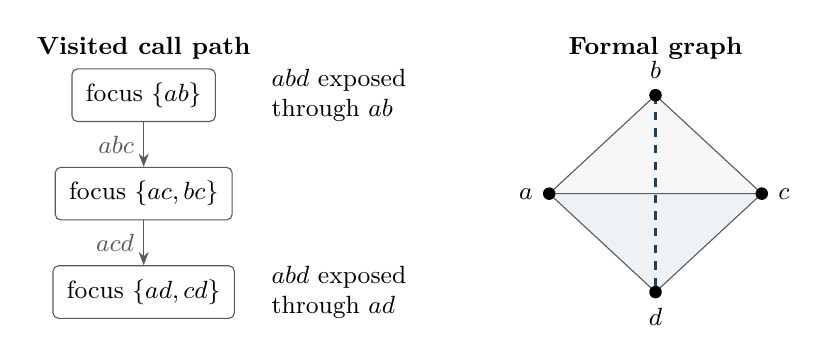
\begin{tikzpicture}[x=1cm,y=1cm,
 call/.style={draw=black!65,rounded corners=2pt,fill=white,
               inner sep=5pt,font=\small},
 vertex/.style={circle,fill=black,inner sep=1.6pt},
 every label/.style={font=\small}]
\node[font=\small\bfseries] at (0,.6) {Visited call path};
\node[call] (root) at (0,0) {focus $\{ab\}$};
\node[call] (first) at (0,-1.25) {focus $\{ac,bc\}$};
\node[call] (second) at (0,-2.5) {focus $\{ad,cd\}$};
\draw[-{Stealth},black!65] (root)--node[left,font=\small] {$abc$} (first);
\draw[-{Stealth},black!65] (first)--node[left,font=\small] {$acd$} (second);
\node[font=\small,align=left,anchor=west] at (1.5,0)
 {$abd$ exposed\\through $ab$};
\node[font=\small,align=left,anchor=west] at (1.5,-2.5)
 {$abd$ exposed\\through $ad$};
\begin{scope}[xshift=6.5cm]
\node[font=\small\bfseries] at (0,.6) {Formal graph};
\coordinate (a) at (-1.35,-1.25);
\coordinate (b) at (0,0);
\coordinate (c) at (1.35,-1.25);
\coordinate (d) at (0,-2.5);
\fill[black!3] (a)--(b)--(c)--cycle;
\fill[linkblue!7] (a)--(c)--(d)--cycle;
\draw[black!65] (a)--(b)--(c)--(a)--(d)--(c);
\draw[dashed,linkblue,thick] (b)--(d);
\node[vertex,label=left:$a$] at (a) {};
\node[vertex,label=above:$b$] at (b) {};
\node[vertex,label=right:$c$] at (c) {};
\node[vertex,label=below:$d$] at (d) {};
\end{scope}
\end{tikzpicture}
\caption{A portion of the visited construction, with distinct labels
written as the formal vertex names. The left arrows are parent--child steps:
traversing $abc$ introduces $c$, and traversing $acd$ introduces $d$.
The solid edges on the right are the corresponding edges of $\Gamma$.
The dashed segment $bd$ denotes an edge between labels in $G$ that is
absent from $\Gamma$. The type $abd$ is exposed at the root through $ab$
and at the last displayed call through $ad$. The collision is therefore detected from
these two candidate lists, regardless of whether either occurrence is
traversed. Other calls are not shown.}
\label{fig:call-graph}
\end{figure}

For a formal vertex $a$, its \emph{ancestral call path} is the path
from a root to the birth call of $a$, including both ends.  Given two
formal vertices $a,b$, let $\Gamma_{a,b}$ be the graph constructed from
the union of their ancestral call paths, using the root edges and
gluings on those paths.  All its calls are visited.  We call $(a,b)$
an \emph{extra-edge witness} if $a,b$ are distinct and nonadjacent in
$\Gamma$, their labels are adjacent in $G$, and $\lambda$ is injective
on $V(\Gamma_{a,b})$.

\begin{lemma}[A geometric witness for a collision]
\label{lem:witness}
If the initial root labels are all distinct, then every occurrence of
$\mathcal C_k$ produces an extra-edge witness.  Moreover, uniformly
over the graphs under consideration,
\begin{equation}
\label{eq:collision-witness}
 \Prb_{\mathrm{ind}}(\mathcal C_k)
 \le O(n^{-1})+
 \Prb_{\mathrm{ind}}(\text{an extra-edge witness exists}).
\end{equation}
The $O(n^{-1})$ term may be omitted when $k=1$.
\end{lemma}

\begin{proof}
First suppose that $\lambda$ is injective on all of $\Gamma$.
If an edge of $G$ between two labels is absent from the formal graph,
its two formal endpoints give the required witness.  It remains to
show that a collision is impossible when there is no such extra edge.

Suppose that a triangle type $T$ is exposed at two calls.  It cannot
occur twice in one list, so the exposing calls are distinct.  Their
responsible focus edges are distinct by property~(ii), and their
images are distinct by injectivity.  Those two edges already represent
all three vertices of $T$, even if neither candidate occurrence is
traversed.  Since there are no extra edges between labels, the three
formal vertices form a triangle of $\Gamma$.  By property~(iv), it is
a gluing triangle.  Its two new edges are focused only at that
gluing's child call, which omits the triangle as its parent.  Its
attachment edge is focused at only one call.  Hence the triangle can
appear in at most one candidate list, a contradiction.

Next suppose that the labels are not injective.  Choose the first
repetition in a construction order with roots first and parents
before children.  The distinct-root assumption means that this
repetition occurs when a new vertex $z$ is attached through an edge
$xy$.  Write $w$ for the earlier vertex with $\lambda(w)=\lambda(z)$.
All earlier labels are distinct.  Property~(i) shows that $x,y,w$ are
distinct and that $\lambda(x)\lambda(w)$ and
$\lambda(y)\lambda(w)$ are edges of $G$.

If either $xw$ or $yw$ is absent formally, it gives an extra edge
among the earlier vertices.  The ancestral paths of its endpoints
are entirely earlier in the construction, so their labels are
injective.  Property~(iii) ensures that the pair remains nonadjacent
in the completed graph.  This is the desired witness.

Otherwise $xyw$ is a formal triangle and hence an earlier gluing
triangle.  There are two possibilities for its latest vertex.
If it is $x$ or $y$, then $xy$ was born at this gluing.  The current
call focusing $xy$ is exactly its birth call, and omits the triangle
$xyw$ as its parent.  It therefore cannot have the proposed child
with the same triangle type.  If the latest vertex is $w$, then $w$
was attached through $xy$.  The children introducing $w$ and $z$
would belong to the same unique call focusing $xy$, and would have
the same triangle type.  That call contains this candidate only once
and traverses it at most once, again a contradiction.  Thus a first
repeated label always produces an earlier extra edge.

Finally, either endpoint of a uniform oriented root has distribution
\[
 \pi(v)=\frac{\deg_G(v)}{2m},
 \qquad \max_v\pi(v)=O(n^{-1}),
\]
by the degree estimate and $2m=n^2p$.  For two independent roots, any
fixed pair of their endpoints coincides with probability
$\sum_v\pi(v)^2\le\max_v\pi(v)$.  There are four pairs to consider;
the two endpoints within each root are distinct.  A union bound
therefore gives the term $O(n^{-1})$ in
\eqref{eq:collision-witness}.
\end{proof}

The root experiment still samples with replacement; we have only
charged its overlaps to the error bound.  The remaining task is to
bound the probability of a visited, injectively labelled pair of call
paths whose two marked vertices have an extra edge.  This uses both
the template estimates for $G$ and the independent-test probabilities.

\section{Counting and visiting collision witnesses}\label{sec:witnesses}

We now bound the probability of the marked path unions furnished by
Lemma~\ref{lem:witness}. The required precision is
$o(D^{-1})$: the probability that two independent root queries both return
true is asymptotic to $q(1)^2\sim(2D)^{-1}$. A collision estimate that merely
tends to zero would not control that second moment.

Throughout this section, $G$ is any graph satisfying
Proposition~\ref{prop:prefix}, and all constants and error estimates are
uniform over such $G$. We work in the independent unfolding. The proof has
two parts. First, the extra edge between the marked vertices makes their
path union rare as a graph embedding. Second, reaching a long prescribed
path requires many earlier candidate queries to fail. We retain the order
of the selected priorities when combining these two bounds.

\subsection{Patterns and their embeddings}

The paths in this section are paths in the \emph{call forest}, not paths
in the formal graph $\Gamma$. Consider the union of the ancestral paths
to the birth calls of two marked formal vertices $a,b$. When the paths
belong to the same rooted tree, let $h$ be their common trunk length and
let $\ell_1,\ell_2$ be the two lengths after the trunk. Length counts
non-root calls. When the paths belong to distinct trees, set $h=0$ and
let $\ell_1,\ell_2$ be their individual lengths. In both cases put
\[
 \ell=h+\ell_1+\ell_2,
 \qquad r=\text{the number of roots used}\in\{1,2\}.
\]
Zero lengths are allowed. A mark born at a root specifies one of its two
formal endpoints.

A \emph{pattern} records these rooted paths, their marks, and the choice
of focus edge at each child step. The named focus edges from
Section~\ref{sec:coupling} give at most two choices at a step. The choices
of roots, the order of the two marked paths, and any marked root endpoints
contribute only an absolute constant. Consequently, for each triple
$(h,\ell_1,\ell_2)$ there are at most
\begin{equation}\label{eq:pattern-count}
 C\,2^\ell
\end{equation}
patterns, for an absolute constant $C$. At a fork the two children each
choose a focus edge; their third vertices will be determined by an
embedding. Thus there is no further length-dependent multiplicity.
Patterns that cannot occur under the query rule may be discarded.



The formal graph $J$ of a pattern starts with $r$ disjoint root edges and
adds two edges and one vertex at each non-root call. In particular,
\[
 v(J)=2r+\ell,\qquad e(J)=r+2\ell.
\]
We consider only patterns whose marks $a,b$ are distinct and nonadjacent
in $J$, and write $J^+=J+ab$. An embedding below is an injective map of
the formal vertices into $V(G)$ that maps every edge of $J^+$ to an edge
of $G$ and respects the named endpoints of each root.

\begin{lemma}[Embedding an extra edge]\label{lem:embeddings}
For every such pattern with $r\in\{1,2\}$ roots and $\ell$ non-root calls,
the number of embeddings of $J^+$ into $G$ is at most
\begin{equation}\label{eq:embedding-bound}
 (2m)^r(2D)^\ell D^{-B}
\end{equation}
for all sufficiently large $n$, uniformly over the pattern and $G$.
\end{lemma}

\begin{proof}
Write $\kappa_n=(1+\log n)^{C_0}$ for the common factor in the two template
bounds of Proposition~\ref{prop:prefix}. Recall that $L=100$, $B=50$,
$p\sim n^{-1/2+\epsilon}$, and $D=np^2\sim n^{2\epsilon}$, where
$\epsilon=1/2000$.

\paragraph{Fewer than $L$ calls.}
Suppose $\ell<L$. Regard $J^+$ as a template with no distinguished
vertices. Order all root vertices first, ordering the endpoints of each
root edge, and then add the other vertices in any parent-first order of
their birth calls. Before adding $ab$, each vertex has at most two
neighbors preceding it. Moreover, the first vertex of any nonempty
vertex subset has no preceding neighbor within that subset. An induced
subgraph on $v>0$ vertices therefore has at most $2v-2$ edges from $J$,
and at most $2v-1\leq 2v$ from $J^+$. Every subgraph satisfies the same
weaker bound $e\leq 2v$. Since $p<1$ and $D>1$ for large $n$, its scaling
is at least
\[
 n^v p^{2v}=D^v\geq1.
\]
The empty subgraph has scaling one. The first template bound gives
\[
 \#\{J^+\hookrightarrow G\}
 \leq \kappa_n n^{2r+\ell}p^{r+2\ell+1}
 =\kappa_n(2m)^rD^\ell p.
\]
Here the template has at most $4+(L-1)=103\leq H_0$ vertices. The
inequality
\[
 pD^B=n^{-1/2+(2B+1)\epsilon+o(1)}
      =n^{-899/2000+o(1)}
\]
shows that $\kappa_np\leq D^{-B}$ for large $n$. This proves
\eqref{eq:embedding-bound} in the short case.

\paragraph{The last $L$ births.}
Suppose $\ell\geq L$. Choose any parent-first ordering of the non-root
calls, with all roots placed first, and let $Z$ be the set of the last
$L$ vertices born. The labels of the preceding vertices can be assigned
in at most
\begin{equation}\label{eq:preceding-labels}
 (2m)^r(2D)^{\ell-L}
\end{equation}
ways. Indeed, there are $2m$ choices for each oriented root, and at most
$2D$ common neighbors of the two endpoints of each subsequent attachment
edge. Discarding restrictions against repeated labels only increases this
bound. We now fix an injective assignment of these preceding labels.

The birth call of every vertex in $Z$ is an ancestor of the birth call
of a marked vertex in $Z$. To see this, every call in the pattern lies
on a path to a marked birth call. Once that path enters the final suffix,
all its subsequent calls lie in the suffix, by the parent-first order.
In particular, at least one endpoint of $ab$ belongs to $Z$.
Figure~\ref{fig:call-paths} illustrates how such a suffix can meet both arms.

\begin{figure}[htbp]
\centering
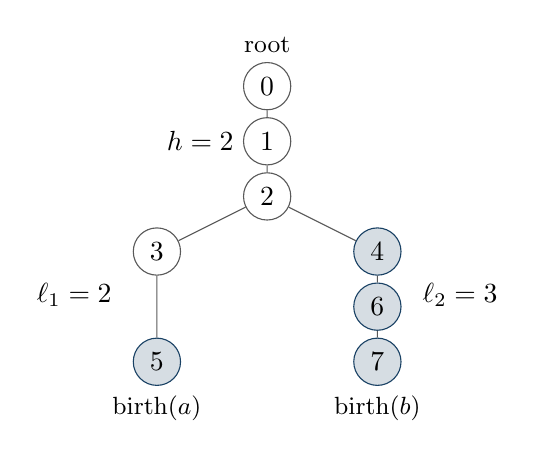
\begin{tikzpicture}[x=1cm,y=1cm,
 call/.style={circle,draw=black!65,fill=white,minimum size=6mm,inner sep=0pt},
 last/.style={call,fill=linkblue!18,draw=linkblue},
 every label/.style={font=\small}]
\node[call,label=above:root] (o) at (0,0) {$0$};
\node[call] (t1) at (0,-.7) {$1$};
\node[call] (t2) at (0,-1.4) {$2$};
\node[call] (a1) at (-1.4,-2.1) {$3$};
\node[last,label=below:$\operatorname{birth}(a)$] (a) at (-1.4,-3.5) {$5$};
\node[last] (b1) at (1.4,-2.1) {$4$};
\node[last] (b2) at (1.4,-2.8) {$6$};
\node[last,label=below:$\operatorname{birth}(b)$] (b) at (1.4,-3.5) {$7$};
\draw[black!65] (o)--(t1)--(t2)--(a1)--(a);
\draw[black!65] (t2)--(b1)--(b2)--(b);
\node at (-.85,-.7) {$h=2$};
\node at (-2.45,-2.65) {$\ell_1=2$};
\node at (2.45,-2.65) {$\ell_2=3$};
\end{tikzpicture}
\caption{A union of two ancestral call paths. Nodes are calls and lines
are parent--child relations, not edges of $G$ or $\Gamma$.
Each non-root call introduces one formal vertex.
The numbers give one parent-first ordering; the last four non-root calls
are shaded. Such a final suffix can occupy both arms and need not be
connected. This small example illustrates the final block used below,
where the proof takes $L=100$.}
\label{fig:call-paths}
\end{figure}

Form a template $(H,I)$ as follows. Its free vertices are $Z$. Retain the
two backward edges of each vertex of $Z$, meaning its edges to the
endpoints of its attachment edge, and retain $ab$. The distinguished set
$I$ consists of all preceding vertices needed as endpoints of these
edges. Include no edges with both endpoints in $I$. We may discard such
constraints because we seek an upper bound on extensions. Thus $I$ is
independent in the template, whether or not its prescribed images have
edges between them in $G$.

The backward edges use at most $2L$ boundary vertices, and the extra edge
uses at most one further boundary vertex. Hence
\[
 |I|\leq2L+1,\qquad v(H)\leq3L+1\leq H_0.
\]
The $2L$ backward edges are distinct, and $ab$ is not one of them.
Every retained edge touches $Z$, so
\begin{equation}\label{eq:terminal-scaling}
 e(H)=2L+1,\qquad
 S(H,I)=n^Lp^{2L+1}=D^Lp
       =n^{-799/2000+o(1)}<1.
\end{equation}

We verify every completion condition needed for the second template
bound. If $U\subsetneq Z$, then
\begin{equation}\label{eq:proper-free-edges}
 e\bigl(H[I\cup U]\bigr)\leq2|U|.
\end{equation}
Indeed, assign each backward edge to its newer endpoint in $Z$. In
$H[I\cup U]$ there are at most two such edges per vertex of $U$.
If \eqref{eq:proper-free-edges} failed, the induced graph would retain
$ab$ and both backward edges of every vertex of $U$. Retaining $ab$
puts every free mark in $U$. Retaining both backward edges of a vertex
also forces the vertex born at its immediate parent call into $U$,
whenever that vertex belongs to $Z$. Indeed, both focus edges at a
non-root parent contain its newly born vertex, so the child's attachment
edge contains that vertex. Repeating this argument backward along each
marked path includes every vertex of $Z$, by the ancestor property just
proved. This would give $U=Z$, a contradiction.

For a proper $U$, \eqref{eq:proper-free-edges} implies
\[
 S\bigl(H[I\cup U],I\bigr)
 =n^{|U|}p^{e(H[I\cup U])}\geq D^{|U|}\geq1.
\]
Every intermediate set of distinguished vertices has the form
$J_0=I\cup U$, with $U\subseteq Z$. Its completion scaling is
\[
 n^{v(H)-|J_0|}p^{e(H)-e(H[J_0])}
 =\frac{S(H,I)}{S(H[J_0],I)}.
\]
For proper $U$ the numerator is less than one by
\eqref{eq:terminal-scaling}, while the denominator is at least one.
For $U=Z$ the ratio equals one. All the required completion scalings are
therefore at most one.

The second template bound now gives at most $\kappa_n$ extensions for the
labels of $Z$. In applying it we may ignore avoidance of previously
assigned vertices outside $I$, again only enlarging the count. Since
$L-B=50>0$ and $D\sim n^{1/1000}$,
\[
 \kappa_n\leq(2D)^L D^{-B}
\]
for all sufficiently large $n$. Multiplying this by
\eqref{eq:preceding-labels} proves \eqref{eq:embedding-bound}.
The threshold for $n$ is uniform: the template order and its
polylogarithmic exponent are fixed independently of the path lengths.
\end{proof}

The embedding bound supplies a factor $D^{-B}$ even when the paths are
arbitrarily long. It remains to sum over their lengths. Counting paths
alone would lose this factor, since a call can have order $D$ children.
The next estimate uses the failures required to reach a prescribed
child, together with the decreasing order of priorities.

\subsection{The probability of visiting prescribed paths}

Fix a pattern and an embedding of $J^+$ \emph{before} exposing any
priorities. The probability that its $r$ used roots have the prescribed
ordered labels is $(2m)^{-r}$. Conditional on this root event, each step
of the pattern specifies one candidate occurrence in a fixed potential
call tree: its focus edge and third vertex determine its triangle.
If these specifications cannot define distinct required children under
the query rule, their visitation probability is zero and they can be
discarded. Otherwise, write $u_y$ for the priority of the selected child
occurrence corresponding to each of the $\ell$ non-root calls $y$.
These are distinct independent uniform coordinates of the unfolding.

Set
\begin{equation}\label{eq:visitation-weights}
 b(t)=q(t)^2=\frac{1}{1+2Dt},\qquad
 C_D=1+2D,\qquad
 \mu=\int_0^1b(t)\,dt=\frac{\log(1+2D)}{2D}.
\end{equation}

\begin{lemma}[Visiting an embedded pattern]\label{lem:visitation}
Conditional on the prescribed ordered root labels, the probability that
all calls in the embedded pattern are visited is at most
\begin{equation}\label{eq:visitation-bound}
 C_D^3\frac{(2\mu)^\ell}{h!\,\ell_1!\,\ell_2!}.
\end{equation}
This includes zero-length segments, with the convention $0!=1$.
\end{lemma}

\begin{proof}
Condition only on the selected priority coordinates $(u_y)$, not on
actual visitation, return values, or previously exposed lists. For all
required calls to be visited, these priorities must decrease along every
required path.

Consider a required non-root call $x$ that has one or two required
children. Its focus is a pair $\{f,g\}$, and its omitted parent triangle
is $T$. Let $t_x$ be the largest priority of its required children.
Define $O_x$ prospectively to be the event that every off-pattern
candidate at $x$ with priority below $t_x$ has a child query returning
false, when that subtree is evaluated hypothetically. Reaching all the
required children necessitates $O_x$. In particular,
\begin{equation}\label{eq:necessary-offpattern}
 \{\text{all required calls are visited}\}
 \subseteq
 \{\text{priorities decrease along the required paths}\}
 \cap\bigcap_x O_x.
\end{equation}
If a required call has two required children, reaching the later child
also requires the earlier selected child to return false. We discard
this additional condition in \eqref{eq:necessary-offpattern}.

Each $O_x$ depends only on subtrees rooted at off-pattern children of
$x$. These subtrees contain none of the selected priority coordinates
and are disjoint for different required calls. In particular, when one
required call is an ancestor of another, the path between them starts
through a selected child, so it does not enter an off-pattern subtree.
The events $O_x$ are therefore independent conditional on $(u_y)$.
This assertion concerns the prospective independent unfolding.

For an off-pattern candidate $S$ attached through focus edge $e$, the
probability that it is not a successful child before $t_x$ is exactly
$1-I_{e,S}(t_x)$. By the product identities of
Proposition~\ref{prop:products},
\begin{equation}\label{eq:offpattern-product}
 \Prb(O_x\mid (u_y))
 =\frac{q_{f,T}(t_x)q_{g,T}(t_x)}
 {\displaystyle\prod_{S\text{ selected at }x}
       (1-I_{e(S),S}(t_x))},
\end{equation}
where $e(S)$ is the unique focus edge contained in $S$.
The denominator removes the one or two selected candidate factors from
the complete product. The product estimate~\eqref{eq:off-pattern-bound}
therefore gives, uniformly in the types and in $t_x\in[0,1]$,
\begin{equation}\label{eq:offpattern-bound}
 \Prb(O_x\mid (u_y))\leq 2b(t_x)
\end{equation}
for all sufficiently large $n$.

We next distribute these factors among the selected child priorities.
At a call with one required child of priority $u$, the bound is $2b(u)$.
At a call with two required children of priorities $u,v$, we use
\[
 \frac{b(\max\{u,v\})}{b(u)b(v)}
 =\frac{1}{b(\min\{u,v\})}\leq C_D.
\]
There is at most one such non-root fork. We ignore the off-pattern
requirements at roots entirely. There are at most two required child
steps leaving roots in total, and inserting their missing factors
$b(u)\geq C_D^{-1}$ costs at most $C_D^2$.
The number of non-root calls with required children is at most $\ell$.
Combining independence, \eqref{eq:necessary-offpattern}, and
\eqref{eq:offpattern-bound}, we obtain the conditional bound
\begin{equation}\label{eq:conditional-visitation}
 C_D^3 2^\ell\prod_y b(u_y)
\end{equation}
when the priorities decrease along the required paths, and zero
otherwise. Every selected priority now carries one factor $b$.
This also covers root marks and empty arms, which introduce no new
priority coordinates.

The selected priorities have joint Lebesgue density one. In integrating
\eqref{eq:conditional-visitation}, retain the order constraints within
the trunk and within each arm, but discard constraints joining different
segments. For a segment of length $j$, symmetry of the product integrand
gives
\[
 \int_{1>u_1>\cdots>u_j>0}\prod_{i=1}^j b(u_i)\,du_1\cdots du_j
 =\frac{\mu^j}{j!}.
\]
The three segments use disjoint coordinates. Their contributions
multiply, proving \eqref{eq:visitation-bound}. Priority ties have
probability zero.
\end{proof}

\subsection{Summing all witnesses}

\begin{proposition}[Uniform collision bound]\label{prop:collision}
Fix $k\in\{1,2\}$ and sample $k$ independent uniform oriented edges of
$G$, with replacement. Execute the independent root queries at threshold
$1$, executing every root regardless of earlier outputs. Let
$\mathcal C_k$ be the event that an actual triangle type is repeated among
all exposed candidate lists, including candidates not traversed. Then
\begin{equation}\label{eq:collision-bound}
 \Prb_{\mathrm{ind}}(\mathcal C_k)
 =O(D^{15-B}+n^{-1})
 =O(D^{-35}+n^{-1})
 =o(D^{-1}).
\end{equation}
The bound is uniform over the graphs in Proposition~\ref{prop:prefix}.
Consequently, by Lemma~\ref{lem:coupling}, the probabilities that all root
queries return true in the finite and independent experiments differ
by at most the same bound.
\end{proposition}

\begin{proof}
Lemma~\ref{lem:witness} reduces a collision to initial root overlap,
which has probability $O(n^{-1})$, or to an injectively labeled marked
path union with an extra edge. For each fixed length triple, multiply
the pattern count \eqref{eq:pattern-count}, the embedding bound
\eqref{eq:embedding-bound}, the root-matching probability $(2m)^{-r}$,
and the visitation bound \eqref{eq:visitation-bound}. The result is at
most an absolute constant times
\[
 D^{-B}C_D^3
 \frac{(8D\mu)^{h+\ell_1+\ell_2}}{h!\,\ell_1!\,\ell_2!}.
\]
For two-tree patterns $h=0$; allowing all triples of nonnegative
integers only enlarges the sum. A union bound over patterns and
embeddings therefore bounds the witness probability by
\begin{align*}
 O\left(D^{-B}C_D^3
   \sum_{h,\ell_1,\ell_2\geq0}
   \frac{(8D\mu)^{h+\ell_1+\ell_2}}{h!\,\ell_1!\,\ell_2!}\right)
 &=O\left(D^{-B}C_D^3\exp(24D\mu)\right)\\
 &=O\left(D^{-B}C_D^{15}\right)
  =O(D^{15-B}).
\end{align*}
All terms are nonnegative; the countable union bound applies to the
almost surely finite evaluations established in
Section~\ref{sec:queries}. The identity
$24D\mu=12\log C_D$ accounts for the exponent $15$.
Finally, $B=50$ and $D\sim n^{1/1000}$ imply
$D^{-35}+n^{-1}=o(D^{-1})$, proving \eqref{eq:collision-bound}.
\end{proof}

We have thus compared the finite continuation with independent root
queries at an error smaller than their two-root success probability.
The first and second terminal moments can now be read directly from
these root-query probabilities.

\section{Terminal moments and the sharp constant}
\label{sec:moments}

We finish by converting the query estimates into moments and then
removing the conditioning on the prefix. Both steps use the uniformity
of all preceding bounds.

Fix a good prefix, and choose $k\in\{1,2\}$ oriented root edges
independently and uniformly with replacement from the $2m$ oriented
edges of $G$. The orientations specify the formal roots and do not
affect the query outputs. In the finite-priority model, each query at
threshold one tests survival of its root edge in the same terminal
graph. Conditional on that graph, its surviving edge fraction is
$F_n/m$, and the sampled roots are independent. Consequently
\begin{equation}\label{eq:finite-moments}
 \Prb(\text{all $k$ finite root queries return true}\mid\text{prefix})
       =\E\left[\left(\frac{F_n}{m}\right)^k
                        \mathrel{\Big|}\text{prefix}\right].
\end{equation}
This identity includes the possibility of repeated sampled edges.
Removing such samples would replace the ordinary second moment by a
different expression.

In the independent unfolding, the trees of the $k$ roots are independent,
even when their edge types coincide. Averaging over the roots gives
\begin{equation}\label{eq:unfolded-moments}
 \Prb(\text{all $k$ independent root queries return true}\mid\text{prefix})
       =\left(\frac1m\sum_{e\in\cE}q_e(1)\right)^k
       =(1+o(1))q(1)^k,
\end{equation}
by Proposition~\ref{prop:unfolding}. Lemma~\ref{lem:coupling} and
Proposition~\ref{prop:collision} bound the difference between
\eqref{eq:finite-moments} and \eqref{eq:unfolded-moments} by
\[
 \Delta_n=O(D^{-35}+n^{-1}).
\]
Since $q(1)^2=(1+2D)^{-1}$,
\begin{equation}\label{eq:relative-error}
 \frac{\Delta_n}{q(1)^2}
    =O(D^{-34}+D/n)=o(1).
\end{equation}
This also controls $\Delta_n/q(1)$, as $q(1)\le1$.

Set $Y_n=F_n/(mq(1))$, using the deterministic $m$ and $D$ from
\eqref{eq:prefix-time}. The two moment identities give, uniformly over
all good prefixes,
\[
 \E[Y_n\mid\text{prefix}]=1+o(1),\qquad
 \E[Y_n^2\mid\text{prefix}]=1+o(1).
\]
Subtracting twice the first identity from the second and adding one
yields
\begin{equation}\label{eq:conditional-l2}
 \E[(Y_n-1)^2\mid\text{prefix}]=o(1)
 \quad\text{uniformly on }\mathcal G_n.
\end{equation}

The normalization has the exact form
\begin{equation}\label{eq:constant}
 a_n:=\frac{mq(1)}{n^{3/2}}
     =\frac{\sqrt D}{2\sqrt{1+2D}}
     =\frac1{2\sqrt{2+1/D}}
     \longrightarrow a:=\frac1{2\sqrt2}.
\end{equation}
In particular $a_n$ is bounded below by a positive constant for large
$n$. Regardless of the prefix, $0\le F_n\le\binom n2\le n^2/2$.
It follows that $(Y_n-1)^2\le Cn$ deterministically. The bad-prefix
contribution therefore satisfies
\[
 \E[(Y_n-1)^2\mathbf1_{\mathcal G_n^c}]
      \le Cn\Prb(\mathcal G_n^c)=o(1).
\]
On $\mathcal G_n$, condition on the complete prefix and use
\eqref{eq:conditional-l2}. We conclude that
\[
 \E[(Y_n-1)^2]\longrightarrow0.
\]
Finally,
\[
 \E\left[\left(\frac{F_n}{n^{3/2}}-a\right)^2\right]
 \le2a_n^2\E[(Y_n-1)^2]+2(a_n-a)^2\longrightarrow0.
\]
Markov's inequality gives the convergence in probability in
Theorem~\ref{thm:main}; Cauchy--Schwarz gives the stated expectation
limit. This completes the proof.

\bibliographystyle{alpha}
\bibliography{references}
\end{document}
